\documentclass[12pt]{article}
\usepackage[a4paper,margin=0.5in,landscape]{geometry}
\usepackage[utf8]{inputenc}
\usepackage{pgfplots}
\usepackage[siunitx]{circuitikz}
\usetikzlibrary{shapes.geometric, arrows}
\usetikzlibrary{automata}
\tikzstyle{bluenode} = [rectangle, rounded corners, minimum width=3cm, text centered, draw=black, fill=blue!30]
\tikzstyle{rednode} = [rectangle, rounded corners, minimum width=3cm, text centered, draw=black,  fill=red!30]
\tikzstyle{brownnode} = [rectangle, rounded corners, minimum width=3cm, text centered, draw=black, fill=brown!30]
\tikzstyle{arrow} = [thick,->,>=stealth]
\author{Mahir Labib Dihan}
\title{My first LaTeX}
\begin{document}
\begin{center}
    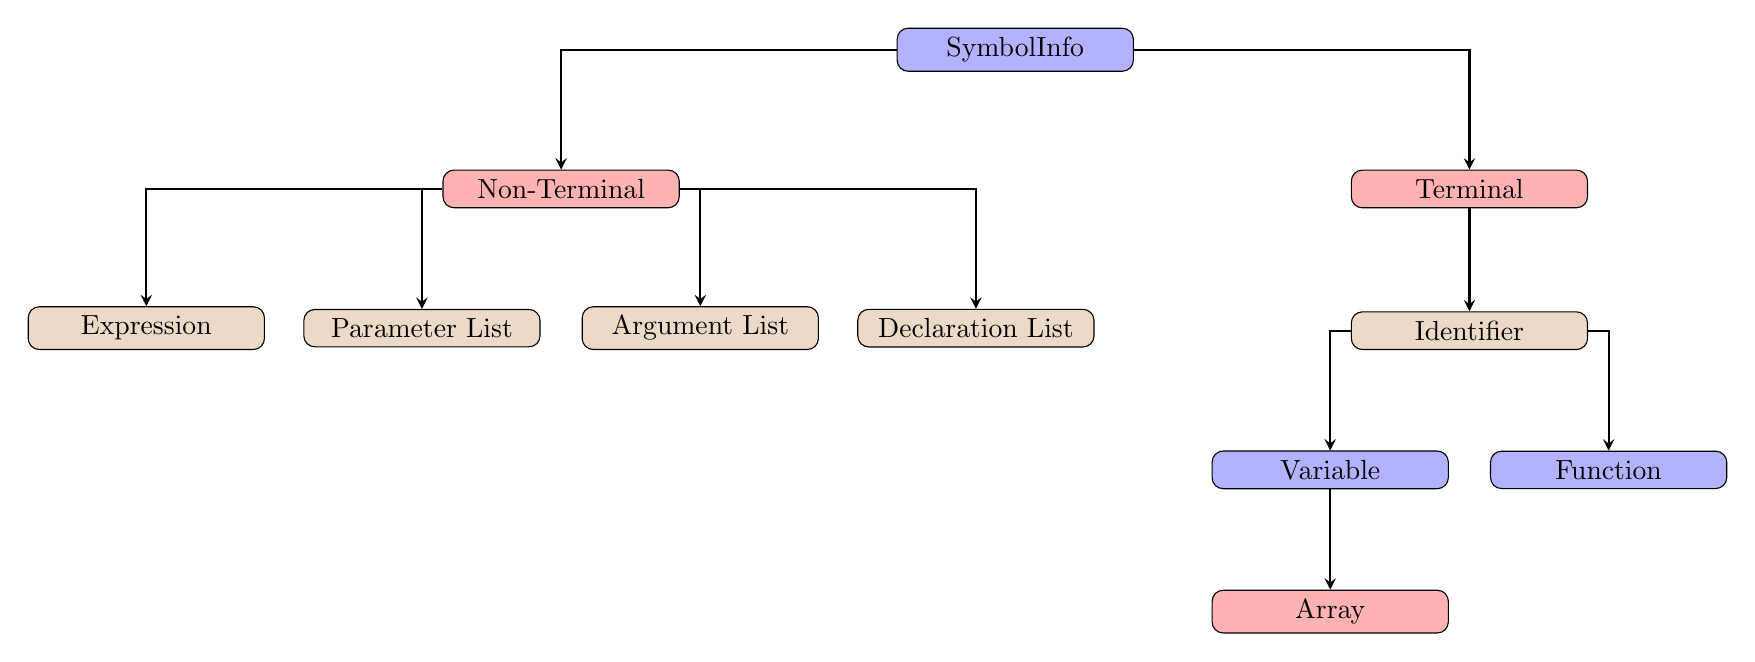
\begin{tikzpicture}[node distance=2.5cm]
        \node (symbol) [bluenode] {SymbolInfo};
        \node (nonterm) [rednode, below left of=symbol, xshift=-4cm] {Non-Terminal};
        \node (term) [rednode, below right of=symbol, xshift=4cm] {Terminal};
        \node (params) [brownnode, below left of=nonterm] {Parameter List};
        \node (expr) [brownnode, left of=params, xshift=-1cm] {Expression};
        \node (args) [brownnode, below right of=nonterm] {Argument List};
        \node (decl) [brownnode, right of=args, xshift=1cm] {Declaration List};
        \node (ident) [brownnode, below of=term,yshift=0.7cm] {Identifier};
        \node (var) [bluenode, below left of=ident] {Variable};
        \node (func) [bluenode, below right of=ident] {Function};
        \node (array) [rednode, below of=var,yshift=0.7cm] {Array};

        \draw [arrow] (symbol) -| (nonterm);
        \draw [arrow] (symbol) -| (term);
        \draw [arrow] (nonterm) -| (expr);
        \draw [arrow] (nonterm) -| (decl);
        \draw [arrow] (nonterm) -| (params);
        \draw [arrow] (nonterm) -| (args);
        \draw [arrow] (term) -- (ident);
        \draw [arrow] (ident) -| (var);
        \draw [arrow] (ident) -| (func);
        \draw [arrow] (var) -- (array);
    \end{tikzpicture}
\end{center}
\end{document}